\documentclass[aspectratio=169]{beamer}

\mode<presentation>
{
  \usetheme{default}
  \usecolortheme{default}
  \usefonttheme{default}
  \setbeamertemplate{navigation symbols}{}
  \setbeamertemplate{caption}[numbered]
  \setbeamertemplate{footline}[frame number]  % or "page number"
  \setbeamercolor{frametitle}{fg=white}
  \setbeamercolor{footline}{fg=black}
} 

\usepackage[english]{babel}
\usepackage[utf8x]{inputenc}
\usepackage{tikz}
\usepackage{courier}
\usepackage{array}
\usepackage{bold-extra}
\usepackage{minted}
\usepackage[thicklines]{cancel}

\xdefinecolor{dianablue}{rgb}{0.18,0.24,0.31}
\xdefinecolor{darkblue}{rgb}{0.1,0.1,0.7}
\xdefinecolor{darkgreen}{rgb}{0,0.5,0}
\xdefinecolor{darkgrey}{rgb}{0.35,0.35,0.35}
\xdefinecolor{darkorange}{rgb}{0.8,0.5,0}
\xdefinecolor{darkred}{rgb}{0.7,0,0}
\definecolor{darkgreen}{rgb}{0,0.6,0}
\definecolor{mauve}{rgb}{0.58,0,0.82}

\title[2018-04-23-dianahep-numba-oamap]{Extending Numba for HEP data types}
\author{Jim Pivarski}
\institute{Princeton University -- DIANA-HEP}
\date{April 23, 2018}

\begin{document}

\logo{\pgfputat{\pgfxy(0.11, 7.4)}{\pgfbox[right,base]{\tikz{\filldraw[fill=dianablue, draw=none] (0 cm, 0 cm) rectangle (50 cm, 1 cm);}\mbox{\hspace{-8 cm}
\includegraphics[height=1 cm]{princeton-logo-long.png}
\includegraphics[height=1 cm]{diana-hep-logo-long.png}}}}}

\begin{frame}
  \titlepage
\end{frame}

\logo{\pgfputat{\pgfxy(0.11, 7.4)}{\pgfbox[right,base]{\tikz{\filldraw[fill=dianablue, draw=none] (0 cm, 0 cm) rectangle (50 cm, 1 cm);}\mbox{\hspace{-8 cm}
\includegraphics[height=1 cm]{princeton-logo.png}
\includegraphics[height=1 cm]{diana-hep-logo.png}}}}}

% Uncomment these lines for an automatically generated outline.
%\begin{frame}{Outline}
%  \tableofcontents
%\end{frame}

% START START START START START START START START START START START START START

\begin{frame}{Can we use Numba for LHC data?}
\vspace{0.5 cm}
Numba provides a smooth transition between high-level tinkering in Python and high-throughput processing, and we've seen a real-world demonstration in XENONnT.

\vspace{0.8 cm}
\textcolor{darkblue}{\Large Can we use it for LHC data?}

\vspace{0.2 cm}
\begin{itemize}
\item Must access ROOT data. \uncover<2->{\textcolor{darkorange}{Solution: uproot, as well as ROOT PR\#943, PR\#1872.}}
\item We need arbitrary length lists of particles per event, not rectangular arrays.
\item Converting all of our events to lists of namedtuples to feed to Numba would be a serious performance hit (memory and throughput).

\vspace{0.2 cm}
\uncover<3->{\textcolor{darkorange}{Solution: object-array mapping (OAMap).}}
\end{itemize}
\end{frame}

\begin{frame}{Object-array mapping (OAMap)}
\vspace{0.5 cm}
By analogy with object-relational mapping (ORM), which translates between classes in object-oriented programming (OOP) and relational tables in databases.

\vspace{0.5 cm}
OAMap translates between OOP objects and low-level, read-only arrays:

\vspace{0.2 cm}
\begin{itemize}
\item[$\rightarrow$] Physicists write arbitrary code on OOP-style objects.
\item[$\rightarrow$] Actual data are stored in arrays (e.g.~TBaskets), never deserialized into objects.
\item[$\rightarrow$] Physicist's function is translated into operations on arrays, not any intermediaries.
\end{itemize}

\vspace{0.2 cm}
\uncover<2->{\textcolor{darkblue}{This is a kind of compilation.} Last year's talks about ``Femtocode'' are this idea in a functional language, but the data representation can be handled on its own.}

\vspace{0.2 cm}
\uncover<3->{In particular, Python is a high-level language that physicists already use, and Numba provides optimized compilation through LLVM.}
\end{frame}

\begin{frame}{Performance tests {\it preceded} design}
\vspace{0.3 cm}
I wanted to make sure that committing to a library (Numba) did not give away performance from the start. I observed no loss in throughput compared to pure C.

\vspace{0.2 cm}
\begin{columns}[t]
\column{0.5\linewidth}
Single-threaded rates of millions of events per second, limited only by trig functions.

\begin{center}
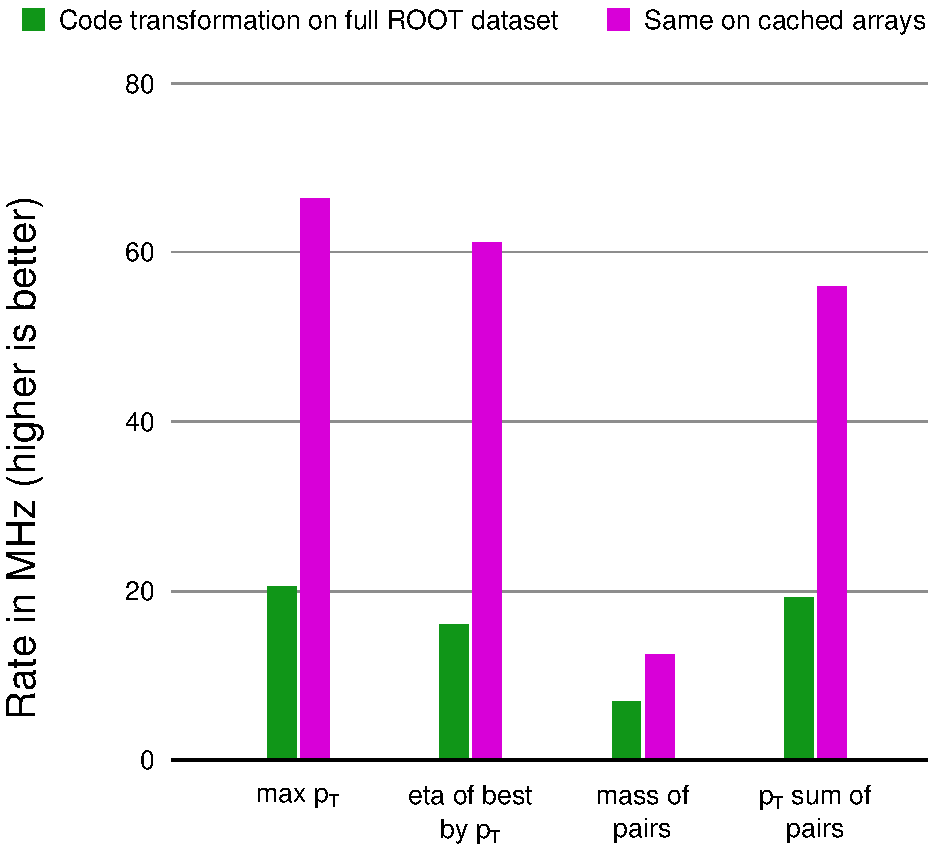
\includegraphics[height=5 cm]{physical-media.pdf}
\end{center}
\column{0.43\linewidth}
Multi-threaded scaling limited only by physical memory bus bandwidth.

\vspace{-0.8\baselineskip}
\begin{center}
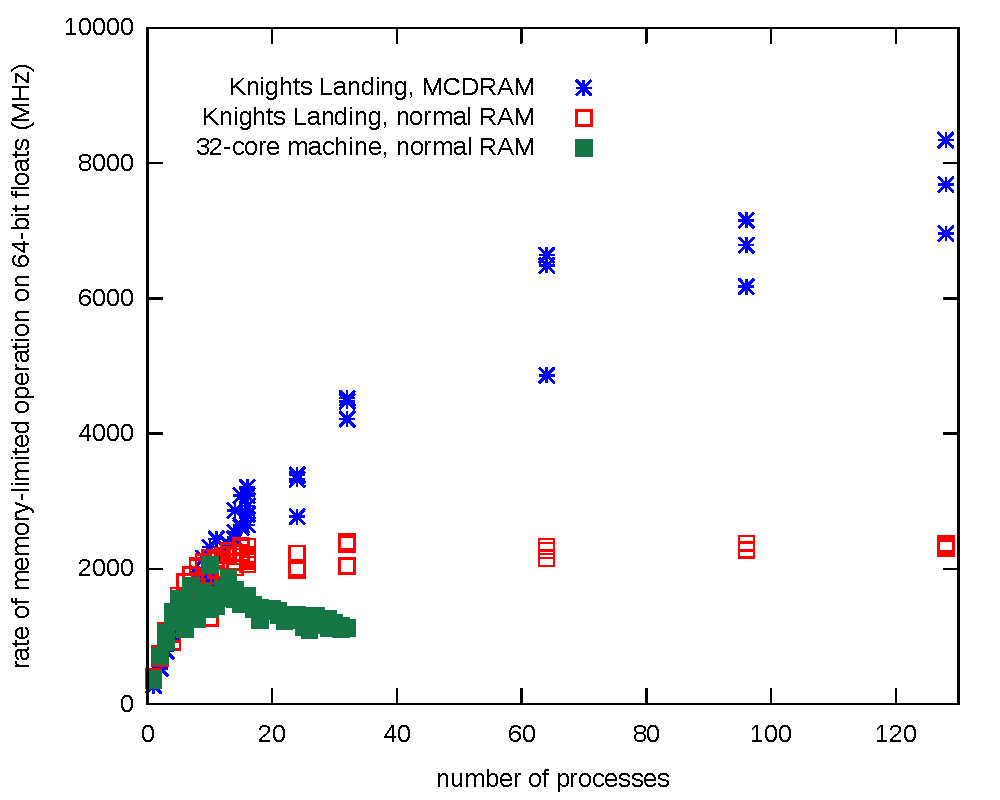
\includegraphics[height=5 cm]{knl-scaling.pdf}
\end{center}
\end{columns}
\end{frame}

\begin{frame}{}
\vspace{0.75 cm}\large

\begin{block}{\LARGE Moral:}
\vspace{0.75 cm}
If we can deliver arrays to main memory and the CPU cache quickly enough,

\vspace{0.35 cm}
and physicists' analyses can be expressed as array operations on sequential data,

\vspace{0.35 cm}
then it can be compiled to run at this scale.
\end{block}

\vspace{0.5 cm}
\begin{center}
\uncover<2->{\textcolor{darkorange}{\Large It's a problem of expressing OOP concepts in arrays.}}
\end{center}
\end{frame}

\begin{frame}{``General enough'' data types}
\vspace{0.35 cm}
\begin{enumerate}
\item \textcolor{darkblue}{\large Primitives:} \uncover<2->{any fixed-width data, such as numbers.}

\item \textcolor{darkblue}{\large Lists:} \uncover<3->{arbitrary-length collections of data with a given type (homogeneous).}

\item \textcolor{darkblue}{\large Unions:} \uncover<4->{set of possible types for heterogeneity (e.g.\ list of ``electrons {\it or} muons'').}

\item \textcolor{darkblue}{\large Records:} \uncover<5->{objects containing a set of typed fields (a.k.a.\ classes or structs).}

\item \textcolor{darkblue}{\large Tuples:} \uncover<6->{fixed-length collections of arbitrary-typed fields (like records with index positions instead of field names).}

\item \textcolor{darkblue}{\large Pointers:} \uncover<7->{objects identified by position in another field. Intended for linking relationships among particles, but also useful for expressing skimmed data as event lists, making non-tree data structures, emulating Arrow/Parquet's ``dictionary encoding'' of categorical strings\ldots}
\end{enumerate}

\vspace{0.2 cm}
The data types and their representations have \textcolor{darkblue}{compositional symmetry:} any type can be plugged into any other type and the array representations follow suit.
\end{frame}

\begin{frame}{Mapping between objects and arrays}
\vspace{0.5 cm}
\textcolor{darkblue}{\large Example:} {\tt List\big(List\big(Record\big(\{"x":\ "char", "y":\ "int"\}\big)\big)\big)}

\vspace{0.25 cm}
\begin{tabular}{r l}
\small logical data & {\tt\scriptsize \textcolor{blue}{[}\textcolor{violet}{[}(\textcolor{darkorange}{a},\textcolor{darkgreen}{1}), (\textcolor{darkorange}{b},\textcolor{darkgreen}{2}), (\textcolor{darkorange}{c},\textcolor{darkgreen}{3}), (\textcolor{darkorange}{d},\textcolor{darkgreen}{4})\textcolor{violet}{]}, \textcolor{violet}{[]}, \textcolor{violet}{[}(\textcolor{darkorange}{e},\textcolor{darkgreen}{5}), (\textcolor{darkorange}{f},\textcolor{darkgreen}{6})\textcolor{violet}{]}\textcolor{blue}{]}, \textcolor{blue}{[]}, \textcolor{blue}{[}\textcolor{violet}{[}(\textcolor{darkorange}{g},\textcolor{darkgreen}{7})\textcolor{violet}{]}\textcolor{blue}{]}\ \textcolor{white}{]}} \\\hline
\small outer list stops & {\tt\scriptsize \textcolor{blue}{[\ \ \ \ \ \ \ \ \ \ \ \ \ \ \ \ \ \ \ \ \ \ \ \ \ \ \ \ \ \ \ \ \ \ \ \ \ \ \ \ \ \ \ \ \ \ \ \ 3,\ \ 3,\ \ \ \ \ \ \ \ \ 4]}} \\
\small inner list stops & {\tt\scriptsize \textcolor{violet}{[\ \ \ \ \ \ \ \ \ \ \ \ \ \ \ \ \ \ \ \ \ \ \ \ \ \ \ 4,\ \ 4,\ \ \ \ \ \ \ \ \ \ \ \ \ \ 6,\ \ \ \ \ \ \ \ \ \ \ \ \ 7\ ]}} \\
\small ``x'' attribute & {\tt\scriptsize \textcolor{darkorange}{[\ \ a,\ \ \ \ \ b,\ \ \ \ \ c,\ \ \ \ \ d,\ \ \ \ \ \ \ \ \ \ \ e,\ \ \ \ \ f,\ \ \ \ \ \ \ \ \ \ \ \ \ g\ \ \ \ \ ]}} \\
\small ``y'' attribute & {\tt\scriptsize \textcolor{darkgreen}{[\ \ \ \ 1,\ \ \ \ \ 2,\ \ \ \ \ 3,\ \ \ \ \ 4,\ \ \ \ \ \ \ \ \ \ \ 5,\ \ \ \ \ 6,\ \ \ \ \ \ \ \ \ \ \ \ \ 7\ \ \ ]}}
\end{tabular}

\vspace{0.5 cm}
\textcolor{darkblue}{\large Transformation rules:}
\begin{itemize}
\item Primitive data at leaves of schema are stored contiguously, with no structure.
\item List structure encoded in a separate array; cumulative number of entries at its level of depth, written at each closing bracket.
\item Other types have similar rules.
\end{itemize}

\vspace{0.2 cm}
\textcolor{darkblue}{\large Proxy objects} only need to know where they are in the schema (compile-time) and where they are in their arrays (integer index at run-time).
\end{frame}

\begin{frame}{Similarity to ROOT and Apache Arrow}
\vspace{0.5 cm}
OAMap transformation rules deliberately resemble those of ROOT and Arrow, so that both can be used as inputs to calculations. With minor modifications, both represent nested data as described on the previous page.

\vspace{-0.2 cm}
\begin{columns}[t]
\column{0.46\linewidth}
\begin{center}
\large \underline{But unlike ROOT,}
\end{center}

OAMap performs calculations on columns in memory. ROOT {\it stores} data in columns (TBranches of TBaskets).

\column{0.46\linewidth}
\begin{center}
\large \underline{But unlike Arrow,}
\end{center}

OAMap performs arbitrary functions (even procedural) on object-like data, rather than a data-frame model.
\end{columns}

\vspace{0.7 cm}
Unlike both, OAMap's focus is on calculation. Any software that provides arrays in the right format may be used as sources.
\end{frame}

\begin{frame}[fragile]{Example}
\small
\begin{minted}{python}
>>> import uproot
>>> import oamap.source.root   # old ROOT interface

>>> url = "http://scikit-hep.org/uproot/examples/HZZ.root"
>>> events = uproot.open(url)["events"].oamap()
>>> events.schema.content["muons"].show()
List(
  starts = 'NMuon',    # schema maps object attributes to array names
  stops = 'NMuon',     # in this case, ROOT TBranch names
  content = Record(
    fields = {         # at all levels of nesting
      'px': Primitive(dtype('float32'), data='Muon_Px'),
      'py': Primitive(dtype('float32'), data='Muon_Py'),
      'pz': Primitive(dtype('float32'), data='Muon_Pz'),
      'energy': Primitive(dtype('float32'), data='Muon_E'),
      'charge': Primitive(dtype('int32'), data='Muon_Charge'),
      'isolation': Primitive(dtype('float32'), data='Muon_Iso')
    }))
\end{minted}
\end{frame}

\begin{frame}[fragile]{Example}
\vspace{0.5 cm}
\small
{\normalsize The dataset ``looks and feels'' like a nested Python list.}
\begin{minted}{python}
>>> events
[<Event at index 0>, <Event at index 1>, <Event at index 2>, ...,
 <Event at index 2418>, <Event at index 2419>, <Event at index 2420>]

>>> events[0].muons
[<Muon at index 0>, <Muon at index 1>]

>>> [x.px for x in events[0].muons]
[-52.899456, 37.73778]
\end{minted}

\vspace{0.5 cm}
{\normalsize But it is generated on demand from arrays. Here's what's loaded now:}
\begin{verbatim}
"NMuon":   array([2, 1, 2, ..., 1, 1, 1], dtype=int32)
"Muon_Px": array([-52.899456,  37.73778,  -0.81645936, ...,
                  -29.756786, 1.1418698,  23.913206  ], dtype=float32)
\end{verbatim}
\end{frame}

\begin{frame}{Compilation with Numba}
\vspace{0.5 cm}
Originally, I was doing AST-to-AST transformations, replacing object references with array references, followed by calling Numba on the result. This required me to do my own type inference. Later, I embedded the objects-to-arrays transformation in the Numba compilation pass itself to gain integration with other Python types for free.

\begin{center}
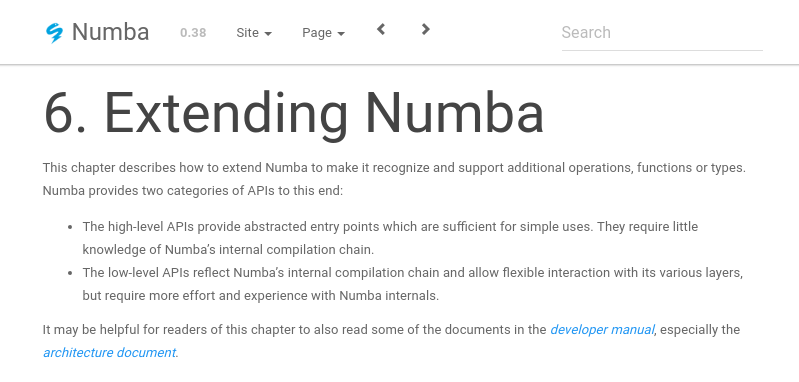
\includegraphics[width=0.8\linewidth]{extending-numba.png}
\end{center}
\end{frame}





\end{document}
